\section{Software Testing}
\label{sec:software-testing}

The process of development in technical product or service requires testing to verify the function of it can do as which had been planned.
In scope of software, testing is the process of executing a program with the intent of finding errors.~\autocite{Myers:2012:Testing:6}
It is about telling the condition of the system (product or service) that passed through a suite of test that mainly define expectation.
The system itself that is being tested is called \ac{SUT}.
These kinds of sofware testing are required to improve code design, increase ability to do refactoring, enhance code documentation, prevent functionality or even performance regression, and much more benefits.
Ordinarily, testing requires to do the following steps:
\begin{inparaenum}[\itshape 1\upshape)]
\item setup,
\item execute,
\item verify, and
\item tear down
\end{inparaenum}
Also commonly test is labeled either red as failed test or green as passed test.

% --------------------------------------------------
\subsection{Unit Testing}

Unit testing is a level of testing independently or individually.
It is written to ensure some or all of particular method can perform it task completely as expected, that carried out in the presence of the stated assertion.
The assurance is when those methods produces the expected output when given the predefined input.
In short, unit testing is regarded from the programmer's actual code perspective, more focused on internal or part functions.

% --------------------------------------------------
\subsection{Integration Testing}

Integration testing or functional testing is mostly a level of testing lots of method that works with each other, so it checks the integration between multiple components.
The assurance is when those methods are working based on what users expecting the software system do.
In short, functional test is regarded from the user's experience perspective, more focused on events and processes that occured when the system is used.

% --------------------------------------------------
\subsection{End-to-End Testing}

End-to-end testing is a level of testing methodology to test particularly complete application flow, performed from start to finish, or end-to-end.
It is mostly done for or in an proposed actual cases that appertain with other components such as external application, database, database, etc.
Therefore it validates the system and interconnected sub-systems.
So all interfaces from frontend to backend are tested.
The assurance is when those cases are performing well based on what the process should be as planned.
For example, a simple \ac{BREAD}-enabled application tested for its ability to browse the data, retrieve and read the data, edit a selected data, add more data, and delete a selected data.

% --------------------------------------------------
\subsection{Automated Testing}

\begin{wrapfigure}{r}{0.5\textwidth}
  \vspace{-20pt}
  \begin{center}
    
\includegraphics[width=5cm]{\dir/include/logo/velocity.png}
  \end{center}
  \vspace{-20pt}
  \caption{Velocity logo}
  \label{fig:velocity-logo}
  \vspace{-10pt}
\end{wrapfigure}

Automated testing of those various types of testing are possible with the help of a testing framework.
Specifically with Meteor framework, there is a testing framework package called Velocity.
Velocity wraps and supports test framework, library, and reporting (that supported in JavaScript) like Mocha, Chai, Jasmine, and much others also for \ac{TDD}, \ac{BDD}, and \ac{ATDD}; making them reactive as well.

% --------------------------------------------------
\subsection{Test First Workflow}

Related inside the \ac{SDLC}, test first workflow or technique is a development process that put the test on the first or initial phase of code implementation.
These kind of \ac{XDD} properly involve the expectation of requirement of the software into the test itself.
It heavily enhance typical developer workflow, which only requires coding, running the code, then complete if the output is as expected.
Basically the things that need to be done are like in \autoref{fig:test-first-workflow}.
The process of it is first to define the expectation based on requirements into the test, the run the test.
Obviously the test will not pass, then this moment is to write or modify the code.
After the test is passed and output is as expected, the particual code or feature that has been done implemented is now complete.

\begin{figure}[!htb]
    \centering
    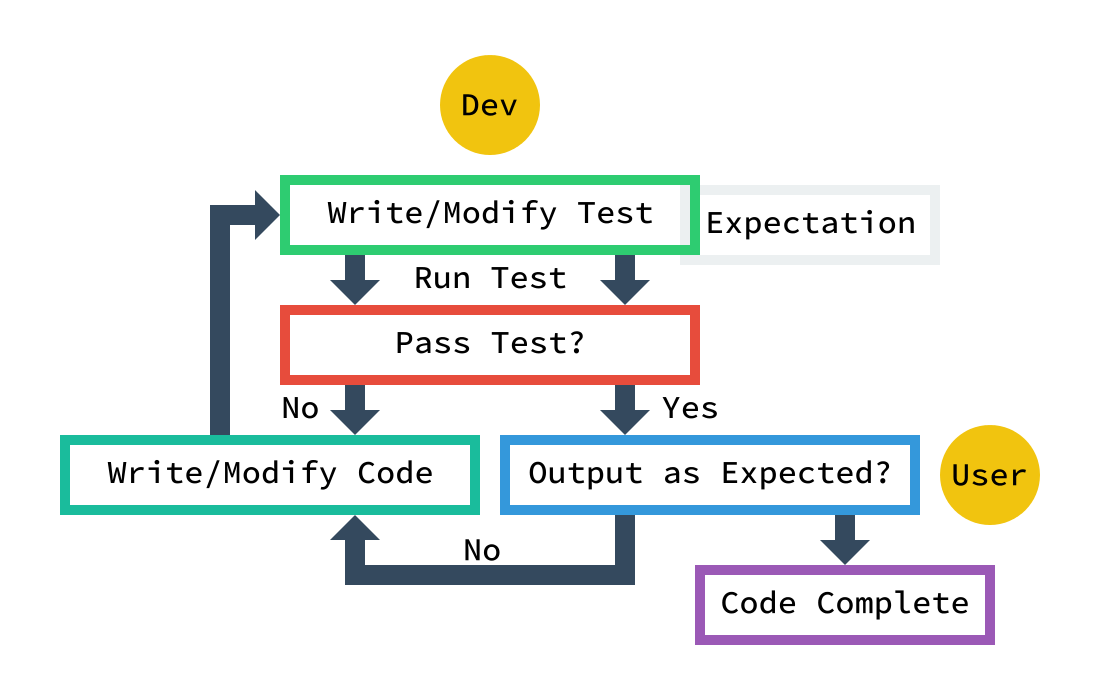
\includegraphics[width=12cm]{\dir/include/test-first-workflow.png}
    \caption{Test First Workflow}
    \label{fig:test-first-workflow}
\end{figure}

% --------------------------------------------------
\subsection{Acceptance Test Driven Development (ATDD)}

More into the test first workflow in particular, there is an \ac{XDD} called \ac{ATDD}.
\ac{ATDD} is an alternative or evolved version of \ac{TDD} and \ac{BDD}, a test-first technique to do software development that is an overall business process rather than just a testing technique.
It aims to involve everyone that needs to be involved throughout the define/build/deploy stages.
\ac{ATDD} is actually a form of \ac{BDD} since it drives the development of the system through its behavior.
The factor that distinguishes \ac{ATDD} is the inclusion of the whole team.
The purpose of this inclusion is to reduce the feedback time which ultimately leads to quicker delivery.~\autocite{Hatoum:2015:MeteorTestingManual}
The process of \ac{ATDD} illustrated in \autoref{fig:atdd}.

\begin{figure}[!htb]
    \centering
    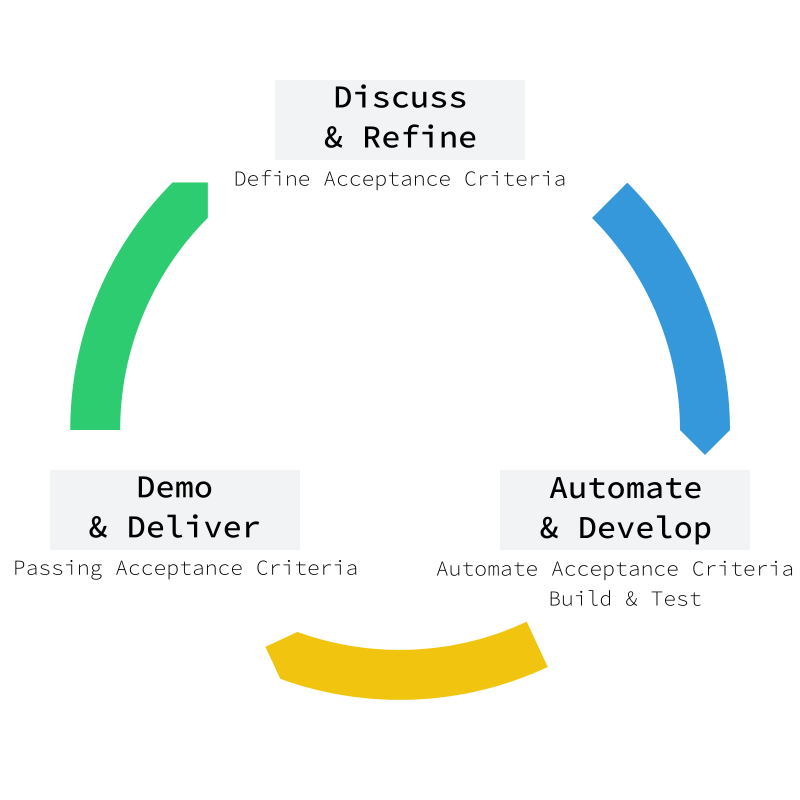
\includegraphics[width=8cm]{\dir/include/atdd.png}
    \caption{ATDD Process}
    \label{fig:atdd}
\end{figure}

The first phase is to define the specifications into a both human-readable and business readable format or \ac{DSL}.
The language commonly used is Gherkin.
Below listing \autoref{lst:gherkin-sample} is an example of a feature file in Gherkin syntax.

\begin{listing}[htb]
\caption{Example of feature file in Gherkin}
\inputminted{ruby}{\dir/include/gherkin-sample.txt}
\label{lst:gherkin-sample}
\end{listing}

After that, automate all of those steps in the scenarios within the test code based on that.
The steps will be implemented as an executable code.

\begin{listing}[!htb]
\caption{Example of an executable feature file}
\inputminted{javascript}{\dir/include/gherkin-executable.js}
\label{lst:gherkin-executable}
\end{listing}

These are qualified as the acceptance tests, drive the value or criteria as described and will be implemented as the actual code once the test requirements are fit.
Lastly, the code is written to implement the code based on the defined tests.
Then after all of the automated process pass the code to the tests and it passed right, the code finally accepted by the test.
When you get to this stage, you expect the acceptance test that you defined and automated in the previous steps to pass. In fact, you can't be at this stage unless the acceptance test passes.
With the process finished and a feature finally completed or delivered, the cycle is restarted again, moving on to the next feature.
It is also possible to refine both test code and implementation code, by refactoring them.
